Salmon have an optimal temperature range for the rate at which they grow. 
If the temperature of their environment goes outside that range, then salmon may change their location of spawning, or time in which they spawn \cite{ADFG-optimal}.
If they do not take either of those options then they may fatigue and die before reaching the spawning location \cite{ADFG-optimal, ADFG-critical}.
So, when temperatures reach a critical point, mortality rates increase significantly, which consequently decreases their growth rate \cite{ADFG-optimal}.
The idea for this section is to use salmon's mortality rate at different temperatures to approximate a growth function, $R(T)$, that is dependent upon temperature, $T$.
While there is little research that scientifically describe the effects of salmon population growth at each individual point in temperature, there are reports that estimate the optimum temperature range as well as critical points.
Dr. Phyllis Weber Scannell wrote an amazing article in 1992 for the ADFG about the optimal temperature ranges for cold water fishes.
In this article, she highlights the optimal range as well as the critical high temperature of sockeye salmon in Alaska~\cite{ADFG-optimal}.
Also, Katherine Carter has published an article that suggests temperatures below $2^{\circ}$C will result in high mortality~\cite{carter2005effects}.\\
\begin{table}[H]
\rowcolors{2}{white!40}{lightgray!40}
    \centering
    \caption{Optimal Temperature Range For Pacific Sockeye Salmon}\label{tab:optimaltemp}
    \vspace{.75cm}
    \begin{tabular}{|c|c|c|c|}
    \hline
         \textbf{Species} & \textbf{Optimal ($^{\circ}$C)} & \textbf{Low ($^{\circ}$C)} & \textbf{High ($^{\circ}$C)}\\
         \hline
         Sockeye & $11-14$ & $<2$ & $>22.2$\\
         \hline
    \end{tabular}
    \vspace{1ex}
    
    {\singlespacing
    % \raggedright 
    *The optimal, critical high and low temperature range for the sockeye salmon species in Alaska \cite{ADFG-optimal, carter2005effects}.\par}
\end{table}
As Dr. Scannel's report states, each researcher estimates slightly different temperature ranges due to a multitude of variables such as: acclimation, age, size, genetic strain, and physiological conditions of the fish~\cite{ADFG-optimal}.
That being said, we will use \tablename~\ref{tab:optimaltemp} to help fit a curve that best illustrates the impact of temperature on the growth of salmon.
Now, Katherine Carter's article explains that at these critical points the population would have a 50\% mortality rate~\cite{carter2005effects}.
So, implying that under ideal conditions and optimal temperatures, 100\% of the salmon population would survive the spawning migration to reproduce, and at the critical temperatures only 50\% would survive.
From \tablename~\ref{tab:optimaltemp} the optimal temperature range is $11-14^{\circ}$C and the critical temperature points are at $2^{\circ}$C and $22.2^{\circ}$C, which can be observed on the graph below.
\begin{figure}[H]
    \centering
    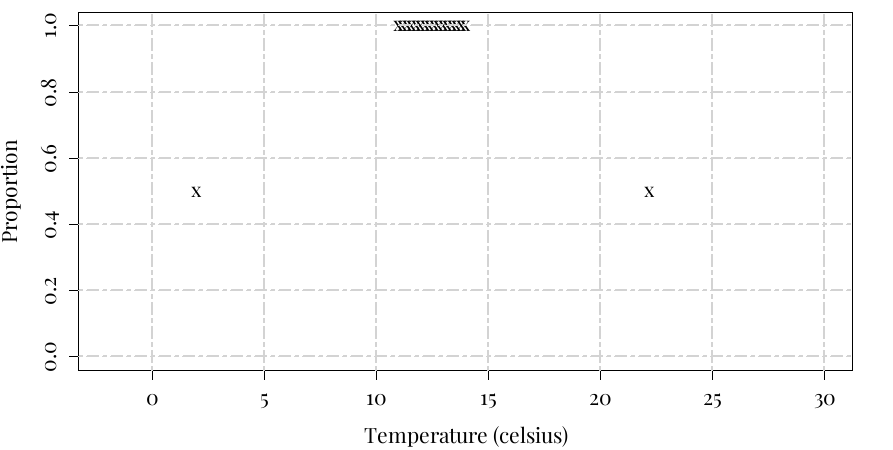
\includegraphics[width=14cm]{Pictures/Salmon Pop/salmon repo model/proportion survival.png}
    \caption{This plot shows the survival rate at the optimal temperature range and the critical temperature points based on \tablename~\ref{tab:optimaltemp}.}
    \label{fig:reproductionpoints}
\end{figure}
Given that the optimal range is rather large, developing a function to approximate these data points will be rather difficult.
The growth rate cannot drop below 0, which implies that we should be looking at a function displayed below.
\begin{equation}\label{eq:reposquared}
    P(T) = \frac{1}{1+c(T-T_{opt})^2}
\end{equation}
Where $T_{opt}$ is the average of the optimal temperature range $12.5^{\circ}$C. $T$ will represent temperature in Celsius and $c$ is a constant that will be calculated to stretch the function horizontally as shown below.
\begin{figure}[H]
    \centering
    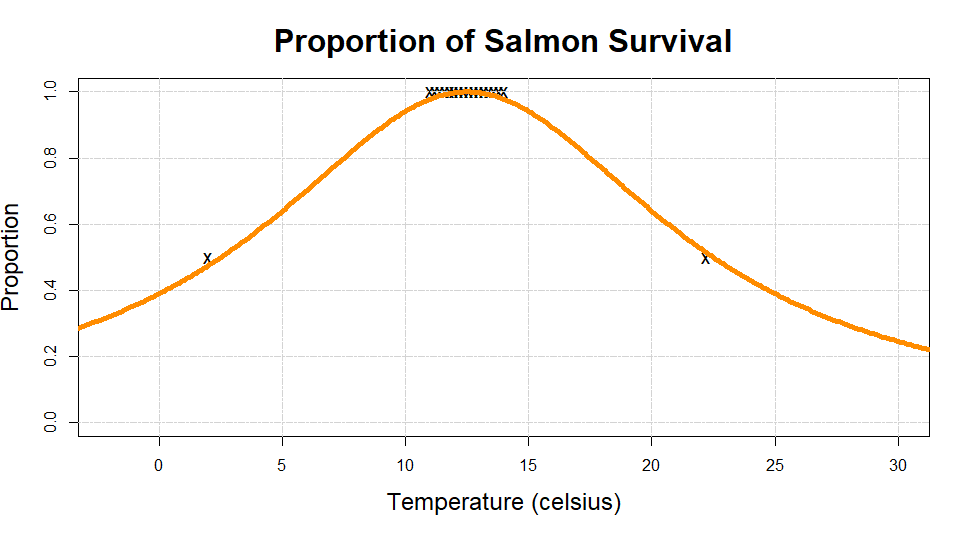
\includegraphics[width=14cm]{Pictures/Salmon Pop/salmon repo model/repo function plot squared.png}
    \caption{This figure represents the data estimated using \equationautorefname~\eqref{eq:reposquared} where $c=0.01$.}
    \label{fig:reporductioncurve2}
\end{figure}
The main issue with using \equationautorefname~\eqref{eq:reposquared} is the optimal range could be better represented by changing the power of 2 in the denominator to a power of 4, which will widen the curve while maintaining a steep decent as the temperature escapes the optimal region. Currently at the limits of the optimal temperature range the survival proportions are $0.978$, which according to the article mentioned earlier should be closer to 1. The below equation fixes this issue by introducing the denominator being to the power of 4 instead of 2.
\begin{equation}\label{eq:repo4th}
    P(T) = \frac{1}{1+c(T-T_{opt})^4}
\end{equation}
Where $c=0.0001$ in order to control the spread of the curve.

\begin{figure}[H]
    \centering
    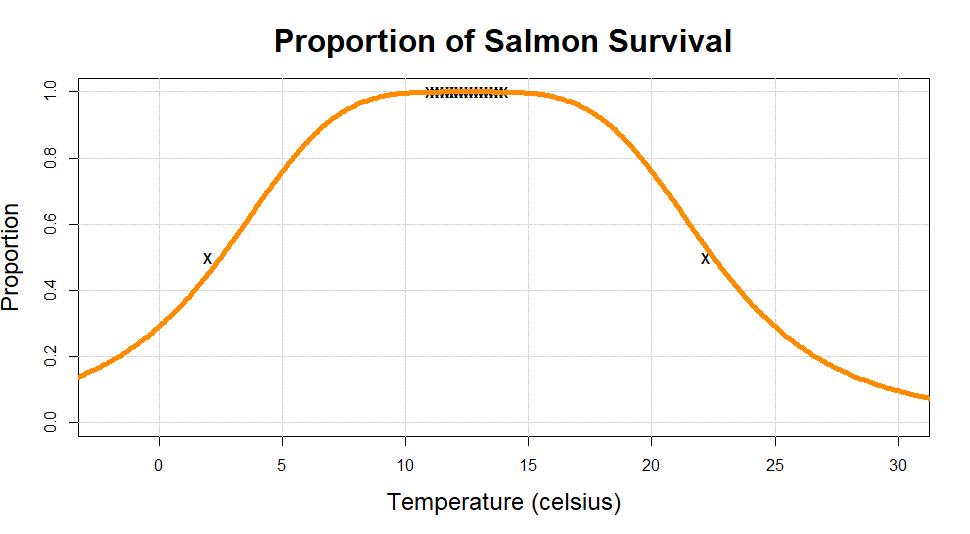
\includegraphics[width=14cm]{Pictures/Salmon Pop/salmon repo model/repo curve 4.png}
    \caption{This figure represents the data estimated using \equationautorefname~\eqref{eq:repo4th} where $c=0.0001$.}
    \label{fig:reporductioncurve4}
\end{figure}
This is a better fit for the optimal temperature range because the survival proportions are now really close close to 1. 
At the limits of the optimal range the survival proportions are $0.9995$, which is approximately 1.
During the salmon migration of 2004, Weaver Creek sockeye salmon experience a drastic rise in water temperature, which resulted in a higher than usually mortality rate~\cite{farrell2008pacific}.
According to Anthony P. Farrell, temperatures were around $20.4^{\circ}$C and that 30\% of the salmon population did not make it to the spawning location due to the excessive heat~\cite{farrell2008pacific}.
Now, using \equationautorefname~\eqref{eq:repo4th}, and letting $T=20.4$ we get $R(20.4)=0.7197$.
This means the we estimate approximately a 72\% survival rate for the salmon migrating to their spawning locations.
This also reveals a mortality rate of approximately 28\% which close to Anthony P. Farrell's estimation.

So far, this reproduction function has just been estimating the proportion of salmon that would reproduce for the next iteration.
Looking back at \equationautorefname~\eqref{eq:fishlogistic}, the reproduction rate, $r$, was when temperatures were ideal, or in the optimal range, so by taking the product of $r$ and $R(T)$, we will have the final reproduction function as shown below.
\begin{equation}\label{eq:repo4thwithr}
    R(T) = r_xR(T) = \frac{r_x}{1+c(T-T_{opt})^4}
\end{equation}
Where $c=0.0001$, $T_{opt}=12.5$, and $r=0.32\ln{5}$.
Lastly, we will replace the reproduction rate, $r$ with the reproduction function, $R(T)$, in \equationautorefname~\eqref{eq:fishlogistic}.
\begin{equation}\label{eq:salmonlogisticrepo}
    \frac{dF}{dt} = R(T)F\left(1-\frac{F}{K}\right)
\end{equation}
To see the affect of temperature on the salmon population, we will compare \equationautorefname~\eqref{eq:salmonlogisticrepo} at different temperatures.
\begin{figure}[H]
    \centering
    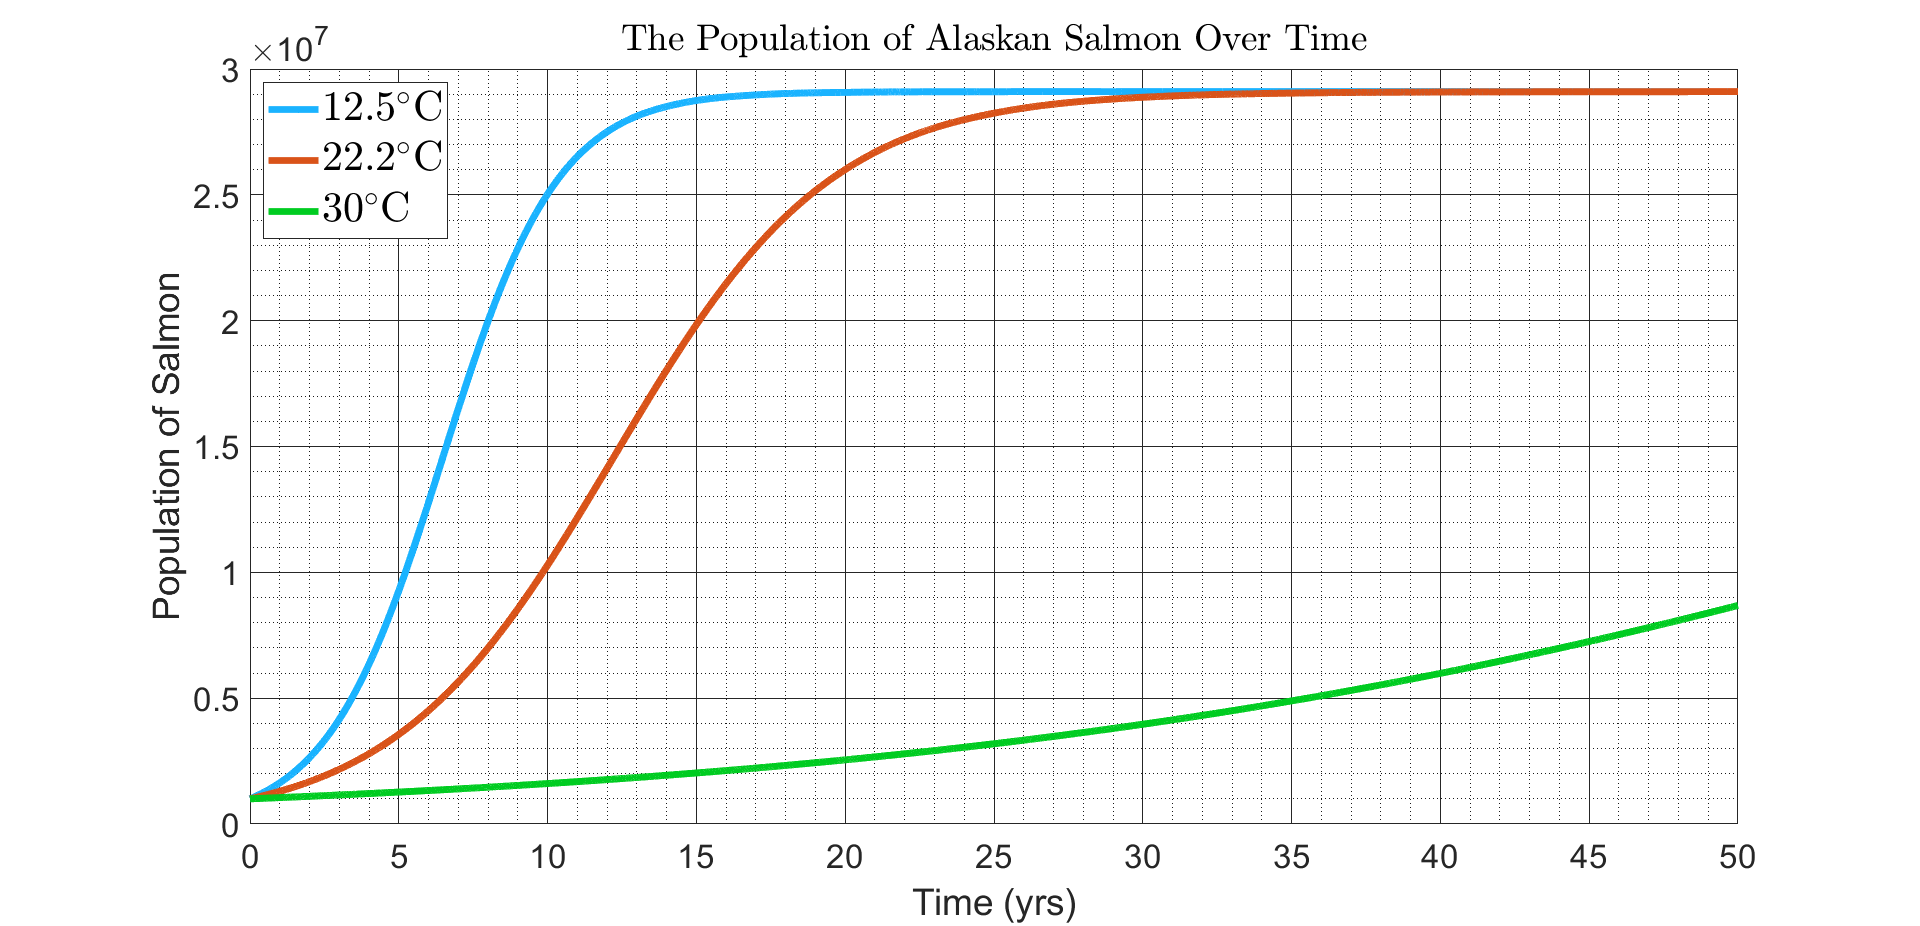
\includegraphics[width=14cm]{Pictures/Salmon Pop/Salmon at 3 dif temps.png}
    \caption{These three curves represent the outcome of the reproduction function, \equationautorefname~\eqref{eq:repo4thwithr}. The initial population was set to 1,000,000 and the parameters discussed in \equationautorefname~\eqref{eq:salmonlogistic},~\eqref{eq:fishlogistic}, \&~\eqref{eq:repo4th} were used in the production of these plots.}
    \label{fig:salmonrepocomparison}
\end{figure}
At the optimal temperature, $T=12.5^{\circ}$C, the population grows drastically from 1 million to almost 29.1 million in 20 years as seen in the top graph.
As the temperature moves further away from the optimal temperature, the reproduction of salmon is negatively affected, resulting in a slower growth rate, which can be observed in the middle and bottom graph.
Notice, that as the temperature becomes drastically far away from the optimal temperature, the growth rate slows down significantly. 
By setting the $T=30^{\circ}$C, the salmon population takes nearly 200 years to reach their environmental carry capacity.

By replacing the reproduction rate of salmon with a function dependent upon temperature, we can see the drastic affects on the salmon population as temperature changes.
If we estimate, or predict, how temperature will change with respect to time, then we can apply it to the salmon population model and discuss the change in growth rate over time due to temperature changing at the same time.
In the next section we will discuss the growth of temperature over time and create a function that will predict temperature at any point in time.
Then, we will incorporate our new function into our reproduction function, \equationautorefname~\eqref{eq:repo4th}, to explore the affects on the salmon population.
